\chapter{Теоретическое введение}

\section{Гедонические игры}
Введем определение гедонической игры, которое будем использовать на протяжении всего исследования.\\

Пусть есть множество агентов $\{1,...,N\}$, $\sigma$ - некоторое разбиение агентов на сообщества, $\sigma=\{S_1,...,S_n:\textbf{ }S_i\cap S_j=\emptyset,\textbf{ }i\neq j;\textbf{ }\cup_i S_i=\{1,...,N\}\}$. Агентов будем также называть игроками. Для каждого агента задана функция полезности $u_i(\sigma)$ (или, иначе, функция прибыли), зависящая от текущего разбиения. Пусть агенты могут свободно перемещаться между кластерами. В данной работе \textit{стратегией} игрока будем называть сообщество, которое данный игрок выбирает. Задача состоит в том, чтобы отыскать \textit{оптимальные стратегии} для каждого игрока: то есть, при выборе данной стратегии игрок имеет максимальную прибыль при фиксированных оптимальных стратегиях всех остальных игроков. В данной работе мы будем рассматривать \textit{некооперативные} игры. Это означает, что два или более игрока не могут действовать согласованно, то есть каждый игрок выбирает стратегию, принимая во внимание только собственную прибыль (\textit{"selfish"} players). Результирующее разбиение, в котором никакой игрок не хочет изменить стратегию, и будет искомым разбиением множества агентов на сообщества.\\

Будем называть рассмотренную игру \textit{гедонической}, если функция полезности $u_i$ каждого игрока зависит только от того, какие еще игроки входят в сообщество, которому принадлежит рассматриваемый игрок. При этом разбиение оставшихся вершин на сообщества никак не влияет на прибыль рассматриваемого игрока. С помощью некооперативных гедонических игр можно моделировать множество ситуаций, в которых агенты объединяются в сообщества, исходя из личных интересов. Впервые гедонические игры были введены и проанализированы в этой работе \cite{firsthg}. Большинство работ по гедоническим играм посвящено изучению \textit{равновесия Нэша} (набора оптимальных стратегий игроков, при которых никакой игрок не хочет изменить свою стратегию при фиксированных оптимальных стратегиях других игроков), а также нахождению оптимальных стратегий игроков, доказательству существования или отсутствия равновесия Нэша в различных игровых моделях \cite{core1}, \cite{core2}, \cite{core3}.\\

Чтобы лучше понять, как могут быть устроены гедонические алгоритмы поиска сообществ, рассмотрим примеры конкретных алгоритмов и решаемых ими задач. Как и в метрических алгоритмах кластеризации, количество кластеров в некоторых теоретико-игровых алгоритмах известно заранее, а в других - нет.\\

Кластеризацию первого типа в литературе часто называют "fixed clustering". Приведем пример такого алгоритма, кластеризующего полный взвешенный неориентированный граф. Назовем условно веса ребер графа "расстояниями". Пусть число кластеров известно заранее и равно $k$. В таком случае удобно формировать кластеры вокруг так называемых \textit{центроидов} - представителей каждого из $k$ кластеров. Введем \textit{цену} кластера - сумму расстояний от всех агентов в данном кластере до его центроида. Тогда введем цену $c_v(C)$, которую платит агент $v$ за нахождение в кластере $C$, как цену кластера $C$, разделенную поровну между его агентами. Теперь прибыль игрока можно считать равной $-c_v$. Набор стратегий игрока - $k$ чисел, обозначающих номера кластеров, которые можно выбрать. На каждом шаге игроку $v$ нужно выбрать такой кластер $C$, что величина $c_v(C\cup v)$ минимальна. Оказывается, что агенту нужно минимизировать собственное расстояние до центроида \cite{clusteringhg}. Примером применения такого алгоритма является организация передачи данных между устройствами, минимизирующая энергетические затраты: устройства объединяются в кластеры согласно приведенному алгоритму, и передача данных осуществляется только между агентом и центроидом одного кластера и между центроидами разных кластеров.\\

Кластеризация второго типа имеет еще более широкое применение, так как зачастую количество кластеров заранее неизвестно. Пусть известны только "отношения"\ между агентами - веса ребер графа. Предположим, что между агентами теперь задана метрика: $d:(u, v)\rightarrow [0,1]$. Пусть $d(u, v)$ обозначает "меру различия"\ объектов $u$ и $v$: если $d(u, v)$ близко к нулю, то объекты похожи, а если, напротив, $d(u, v)$ близко к единице, то объекты очень разные. Пусть также каждый агент $v$ имеет вес $w_v$, обозначающий "меру влияния"\ на остальных. Пусть агенты хотят быть в одном кластере с близкими им объектами с большим весом, но отделиться от непохожих на них агентов с маленьким весом. С помощью функции полезности агента можно это учесть \cite{clusteringhg}. Так можно решать любую задачу, в которой, например, агенты хотят объединиться "по интересам"\ , отдалившись от тех, кто на них не похож.\\

Второй пример важен для нас в данной работе, так как мы будем рассматривать именно этот тип кластеризации, когда количество кластеров заранее неизвестно. Кроме того, мы будем использовать похожую функцию полезности, но функция веса ребер графа $d(u, v)$ уже не будет метрикой, и даже не будет определена для всех пар вершин. Соответственно, $d(u, v)$ уже нельзя считать расстоянием. Веса вершин в нашей работе также будут использоваться, но будет рассмотрено большое их количество, и зависеть они будут от топологии графа, чего в рассмотренной выше постановке, использующей всегда полный граф, быть не может. Про веса вершин будет подробно рассказано в следующей части теоретического введения. 

\section{Центральности}

Понимание роли каждого элемента системы является важным шагом в изучении поведения этой системы. Мы будем изучать кластеризацию ориентированных графов (или, иначе, \textit{сетей}) с различной топологией. Если рассматривать ребро графа как некоторую характеристику "влияния"\ одной вершины на другую, то такие величины, как количество in- или out-соседей, веса in- или out-ребер, а также какие-то характеристики соседей вершины, могут дать представление о важности вершины в сети. Такая мера важности вершины графа называется \textit{мерой центральности}. Мер центральности можно ввести очень много. Рассмотрим здесь те, которые будем использовать для определения важности вершин в данной работе. Приведенные меры центральности определены для ориентированных графов.

\subsection{Betweenness}
Эта мера широко используется в социальных сетях \cite{betweenness}. Она основана на предположении о том, что, если человек в некоторой социальной группе имеет "центральное"\ положение, соединяя много пар других людей, то он важен для этой группы. Этот человек может в определенной мере контролировать общение людей, связанных между собой через него. В терминах сети: если вершина лежит на большом количестве кратчайших путей между другими вершинами, то мера центральности этой вершины должна быть высокой. Рассмотрим вершины графа $i$ и $j$. Пусть число всех кратчайших путей (называемых также \textit{геодезическими}) из $i$ в $j$ равно $g_{ij}$. Для каждой вершины графа $k$ обозначим через $g_{ij}(k)$ число кратчайших путей из $i$ в $j$, содержащих $k$. Тогда мера центральности $k$ ($C_B(k)$) вводится следующим образом:
	\begin{equation}
	b_{ij}(k) = \frac{g_{ij}(k)}{g_{ij}},
	\end{equation}
	\begin{equation}
	C_B(k) = \sum_{i<j}b_{ij}(k),
	\end{equation}
где $b_{ij}(k)$ - доля путей передачи информации из $i$ в $j$, на которых содержится $k$. 
	
\subsection{Degree centrality}
В некоторых сетях удобно ввести меру центральности так, чтобы она зависела от степени вершины. Например, рассмотрим распространение инноваций в социальных сетях. Чем больше степень вершины, тем больше вершин могут "заразиться"\ от данной (принять инновацию). В нашей задаче граф ориентированный, поэтому мера центральности вершины будет пропорциональна числу исходящих ребер (out-степени вершины). Обозначим через $d_{max}$ максимальную out-степень вершины в графе. Тогда меру центральности вершины $i$ будем считать так:
	\begin{equation}
	C_d(i) = \frac{\sum_{j\neq i} \delta_{ij}}{d_{max}},
	\end{equation}
	\begin{equation}
	d_{max} = \max_i\{\sum_{j\neq i}\delta_{ij}\},
	\end{equation}
	где $\delta_{ij}=0$, если ребра $i\rightarrow j$ нет, $\delta_{ij}=1$, если ребро $i \rightarrow j$ есть.\\
	
	Также рассмотрим \textit{weighted} (взвешенную) degree-центральность, в которой важность вершины будет зависеть не только от числа исходящих ребер, но и от их веса (например, в уже рассмотренной социальной сети наличие связи не говорит о том, что информация точно будет передана; вместо этого, можно задать вес ребра как некоторую величину, оценивающую вероятность передачи информации по ребру). Теперь нам потребуется максимальная по всем вершинам сумма весов исходящих ребер в графе $w_{max}$. Мера центральности вершины $i$:
	\begin{equation}
	C_{wd}(i) = \frac{\sum_{j\neq i} \delta_{ij}\cdot w_{ij}}{w_{max}},
	\end{equation}
	\begin{equation}
	w_{max} = \max_i\{\sum_{j\neq i}\delta_{ij}\cdot w_{ij}\},
	\end{equation}
	где $w_{ij}$ - вес ребра $i \rightarrow j$.
	
	\subsection{Closeness}
	Эта мера центральности, как нетрудно понять из названия, характеризует "близость"\ вершины ко всем остальным вершинам графа. Пусть $d_{ij}$ - число ребер в кратчайшем пути от вершины $i$ до вершины $j$. Тогда рассмотрим меру:
	\begin{equation}
	D_c(i)=\sum_{j\neq i} d_{ij}.
	\end{equation}
	Указанная величина имеет противоположный смысл: чем меньше сумма кратчайших расстояний от данной вершины до всех остальных, тем более она "центральна". Значит, меру центральности вершины $i$ можно ввести как величину, обратную $D_c(i)$:
	\begin{equation}
	C_c(i) = \frac{1}{\sum_{j\neq i} d_{ij}}.
	\end{equation}
	В уже рассмотренной задаче распространения инноваций closeness-центральность может характеризовать скорость распространения инновации по сети от заданного узла.
	
	\subsection{PageRank}
	Центральность вершины в ориентированном графе можно измерить с помощью известного алгоритма ранжирования страниц, соответствующих некоторому поисковому запросу \cite{pagerankcent}. Согласно алгоритму PageRank \cite{pagerank}, вес страницы А тем больше, чем больше вес страниц В, на нее ссылающихся. Также чем больше страниц В ссылаются на данную страницу А, тем больше вес страницы А. На основе этих соображений можно определить центральность вершины $i$ в ориентированном взвешенном графе:
	\begin{equation}
	w_i = \alpha \sum_j A_{ji} \frac{w_j}{d_j^{out}}+\beta
	\end{equation}
	где $w_i$ - вычисляемый вес вершины $i$, $\beta$ - коэффициент "затухания"\ (необходим для того, чтобы циклы в графе не "стягивали"\ на себя всю центральность), $w_j$ - вес вершины $j$, являющейся in-соседом $i$, $d_j^{out}$ - out-степень вершины $j$, $A_{ji}$ - вес ребра $j\rightarrow i$ (считается равным нулю, если ребра нет).
	
	\subsection{Другие веса}
	В данной работе будут также использованы веса вершин, не являющиеся мерами центральности.
	
	\begin{enumerate}
		\item Одинаковые веса для всех вершин.\\
		Для теоретического исследования алгоритма потребуется устанавливать веса всех вершин равными $\frac{1}{2}$.
		
		\item Случайные веса.\\
		Важности вершин в реальных задачах не всегда зависят от топологии графа: они могут быть получены, например, на основании экспертного мнения. Однако, кластеризация такого графа все еще будет зависеть от топологии. Для изучения такого случая можно присвоить вершинам случайные веса, лежащие на отрезке $[0,1]$.
	\end{enumerate}

\section{Модулярность}
\textit{Модулярностью} будем называть меру качества кластеризации графа. В алгоритмах, использующих модулярность, ищется максимизирующее модулярность разбиение вершин графа на кластеры \cite{modularity}. Модулярность определяется по-разному для ориентированных и неориентированных графов. Мы будем сравнивать результаты работы нашего алгоритма с алгоритмами, максимизирующими модулярность, чтобы попробовать понять его свойства.\\

Введем вначале определение модулярности для неориентированного графа, а затем обобщим его. Пусть задан неориентированный граф $G=(V,E)$, $|V|=N$, $|E|=m$. Пусть фиксировано разбиение вершин  $\sigma=\{S_1,...,S_n:\textbf{ }S_i\cap S_j=\emptyset,\textbf{ }i\neq j;\textbf{ }\cup_i S_i=\{1,...,N\}\}$. Модулярность оценивает вероятность существования ребра между двумя вершинами в неориентированном графе в сравнении с вероятностью его появления в случайной графической модели с тем же распределением по степеням вершин. Например, если ребро оказывается между двумя вершинами с большой степенью, то это неудивительно, и такое ребро вносит небольшой вклад в модулярность. Если же ребро появляется между вершинами с небольшой степенью, то это маловероятное событие, а значит, оно вносит в модулярность больший вклад. Модулярность $q(\sigma)$ разбиения $\sigma$ можно ввести следующим образом:
\begin{equation}
q(\sigma)=\sum_{i=1,\dots,n} [\frac{|E(S_i)|}{m}-(\frac{\sum_{v\in S_i} deg(v)}{2m})^2],
\end{equation}
где $|E(S_i)|$ - число ребер в подграфе, индуцированном подмножеством вершин $S_i$, $deg(v)$ - степень вершины $v$, $n$ - число сообществ в разбиении $\sigma$.\\

Модулярность разбиения на сообщества ориентированного графа можно найти в работах \cite{newmandir}, \cite{louvain}. Для начала, модулярность разбиения неориентированного графа можно переписать в виде:
\begin{equation}
q(\sigma) = \frac{1}{2m}\cdot \sum_{i,j} (A_{ij}-\frac{d_id_j}{2m})\cdot\delta(S_i, S_j),
\end{equation}
где $A_{ij}$ - вес ребра между $i$ и $j$, $d_i$ - степень вершины $i$, $d_j$ - степень вершины $j$, $\delta(S_i, S_j)=1$, если $i$ и $j$ лежат в одном сообществе, и $\delta(S_i, S_j)=0$, если $i$ и $j$ лежат в разных сообществах. Теперь эту модулярность можно адаптировать для ориентированного графа. Если вершина $i$ имеет небольшую in-степень, а вершина $j$ имеет небольшую out-степень, то ребро $j \rightarrow i$ гораздо менее вероятно, а значит, должно вносить гораздо больший вклад в модулярность, чем ребро $i \rightarrow j$. Формула приобретает такой вид:
\begin{equation}
q_d(\sigma) = \frac{1}{2m}\cdot \sum_{i,j} (A_{ij}-\frac{d_i^{in}d_j^{out}}{2m})\cdot\delta(S_i, S_j),
\end{equation}
где $d_i^{in}$ - in-степень вершины $i$, $d_j^{out}$ - out-степень вершины $j$. \\

\section{Модели случайных графов}
Для изучения свойств алгоритма необходимы \textit{ансамбли случайных графов}. В данной работе используются две модели: \textit{модель Эрдеша-Реньи} и \textit{модель Барабаши-Альберт}.

\subsection{Модель Эрдеша-Реньи}
Рассмотрим $N$ вершин, не соединенных изначально ребрами. Случайным будет множество ребер графа. В модели Эрдеша-Реньи с заданной заранее вероятностью $p=p(N)$ между парой вершин проводится ребро. В случае неориентированного графа рассматриваются неупорядоченные пары вершин, а в случае ориентированного - упорядоченные. Известно, что при $p=\frac{c\cdot \log N}{N}$, где $c>1$, граф почти всегда связен, а если $c<1$, то граф почти всегда не является связным \cite{randomgraphs}.

\subsection{Модель Барабаши-Альберт}
Модель Барабаши-Альберт появилась как способ описания роста интернета, представленного в виде веб-графа. Авторы считали, что в каждый момент времени появляется новый сайт, и этот сайт ставит фиксированное количество ссылок на своих предшественников. Он предпочтет сослаться прежде всего на тех, кто и так уже популярен. Можно допустить, что вероятность, с которой
новый сайт поставит ссылку на один из прежних сайтов, пропорциональна числу уже имевшихся на тот сайт ссылок. Это модель так называемого \textit{предпочтительного присоединения}.\\

В оригинальных работах авторов представлены только модели генерации неориентированных графов по изложенной схеме, но в 2003 году была предложена модель генерации ориентированного графа по похожей схеме с сохранением степенного закона (вероятность того, что вершина в графе Барабаши-Альберт имеет степень $d$, порядка $1/d^3$) \cite{barabashi2003}. В этой модели вершина появляется не на каждом шаге, а добавляется с вероятностью $\alpha\in [0,1]$. С вероятностью $1-\alpha$ новые вершины не появляются. При этом, если вершина была добавлена, то c вероятностью $\beta$ новая вершина ссылается на одну из старых, и вероятность сослаться на конкретную вершину пропорциональна входящей степени старой вершины. С вероятностью $1-\beta$ одна из старых вершин ссылается на новую, и вероятность выбора одной из старых вершин пропорциональна ее исходящей степени. Если вершина не была добавлена, то ребро проводится между двумя старыми вершинами, при этом вероятность выбора точки начала пропорциональна исходящей степени, а конца - входящей степени. Такую модель предлагается использовать для генерации ориентированного графа.

\section{Веса ребер}
Мы знаем, как сгенерировать случайную топологию ориентированного графа и как определить важности его вершин. Осталось понять, как задать веса ребер. В данной работе использовались три подхода:

\begin{enumerate}
	\item Случайные веса.\\
	Веса выбирались из равномерного распределения на отрезке $[0,1]$, из нормального распределения с параметрами $\mu=1/2$, $\sigma^2=1/6$.
	\item Статические веса.\\
	Веса всех ребер одинаковы и равны $1/2$.
	\item Индекс Жаккара.\\
	Вес, равный индексу Жаккара, единственный из рассматриваемых зависит от топологии. Индекс Жаккара определен для произвольных конечных множеств, мы применим его к множествам соседей вершины. Можно понимать его как степень "похожести"\ вершин:
	\begin{equation}
	J(u,v)=\frac{|E(u)\cap E(v)|}{|E(u)\cup E(v)|}.
	\end{equation}
	Чем больше у вершин общих соседей, тем выше вес ребра между ними. Для ориентированных графов будем рассматривать только out-соседей.
\end{enumerate}

\section{Статистический анализ данных}
Статистический анализ данных применялся в работе для анализа полученных распределений, оценки их параметров и интерполяции зависимостей. Приведем основные методы, использованные в работе.

\subsection{Оценка максимального правдоподобия}
Пусть есть выборка $\mathbf{X}=\{x_1,\dots, x_n\}$ из некоторого распределения $f(\theta, x)$, где $\theta$ - неизвестный параметр. Тогда $x_i$ - реализации случайной величины из распределения $f(\theta, x)$. Требуется оценить $\theta$. Определим \textit{функцию правдоподобия} выборки:
\begin{equation}
L(\theta, \mathbf{X})=\prod_{i} f(\theta, x_i). 
\end{equation}
\textit{Оценкой максимального правдоподобия} (ОМП) параметра $\theta$ называется число $\hat{\theta}$, при котором функция правдоподобия для данной выборки достигает максимума.\\

Обычно ОМП ищут из уравнения:
\begin{equation}
\frac{\partial L(\theta, \mathbf{X})}{\partial \theta} = 0.
\end{equation}
Этого достаточно, если функция $-L(\theta, \mathbf{X})$ выпукла по $\theta$.\\

Нам понадобятся оценки максимального правдоподобия параметров нормального распределения: $\mu$ и $\sigma^2$, и параметра $\lambda$ распределения Пуассона. Они равны, соответственно:
\begin{equation}
\mu = \frac{1}{n}\sum_i x_i = \mathbf{\bar{X}},
\end{equation}

\begin{equation}
\sigma^2 =  \frac{1}{n}\sum_i (x_i-\mu)^2 = S^2,
\end{equation}

\begin{equation}
\lambda = \frac{\sum_i x_i}{n} = \mathbf{\bar{X}}.
\end{equation}

\subsection{Проверка нормальности данных}
Для проверки нормальности распределений использованы статистические тесты и QQ-график. Использовались критерии Шапиро и Харке-Бера.\\

Критерий Шапиро разработан специально для проверки нормальности распределения малых выборок, численностью от трех до пятидесяти элементов \cite{shapiro}.\\

Тест Харке-Бера \cite{jarqueber} является асимптотическим тестом, то есть применим к большим выборкам. Статистики, используемые в данных критериях, можно посмотреть в приведенных статьях.\\

Графики квантиль-квантиль (QQ) — это графики, на которых квантили из двух распределений расположены относительно друг друга. Если данные согласуются с проверяемым распределением, точки выстроятся на линии, проходящей под углом 45 градусов. Иначе, точки отклонятся от базовой линии. QQ-график можно применять не только для проверки нормальности распределения, но и для сравнения с любым другим распределением.

\subsection{Регрессия}
Для интерполяции полученных зависимостей использовался регрессионный анализ: аппроксимация реальной зависимости целевой переменной $Y$ от "предикторов"\ $x_1,\dots,x_p$ с помощью модели $Y=f(x_1,\dots,x_p)+\varepsilon$, где $\varepsilon$ - случайная ошибка. Оценки параметров производились с помощью метода наименьших квадратов, основанного на минимизации суммы квадратов отклонений ответов модели от полученных в ходе эксперимента результатов.

\chapter{Алгоритм}
Напомним, что мы решаем задачу поиска сообществ во взвешенном ориентированном графе с заданной топологией с помощью теоретико-игрового алгоритма. В данной работе вершины графа рассматриваются как агенты, ребра - как связи между агентами. И вершинам, и ребрам присваиваются веса - числа от 0 до 1. Вес ребра $u\rightarrow v$ можно интерпретировать как степень желания агента $u$ находиться в одном сообществе с агентом $v$: чем больше этот вес, тем больше прибыль будет у $u$, если он окажется в сообществе с $v$. Вес вершины отражает степень ее "важности"\ (или "влияния"\ на другие вершины). Будем считать, что чем больше вес вершины, тем сильнее другие вершины хотят объединиться с ней, даже если вес соответствующего ребра не слишком большой. На основе этих предположений позже будет определена функция полезности.\\

Каждый агент имеет функцию полезности, которую в процессе работы алгоритма старается увеличить. Как уже было отмечено, мы будем исследовать гедоническую игру на графе. В нашем случае это будет означать, что фиксированное сообщество для вершины тем лучше, чем больше ее соседей, с которыми она хочет находиться (а это желание определяется весом соответствующих ребер и вершин), оказывается в этом сообществе. Также игра \textit{некооперативная}: все игроки действуют только с целью улучшить собственную прибыль. Последнее утверждение верно, если понимать под стратегией \textit{номер выбранного кластера}. Вообще, игра называется \textit{кооперативной}, если игроки могут выбирать стратегии, основываясь на какой-то общей выгоде, то есть, могут "действовать сообща". В нашем алгоритме будет реализована возможность \textit{непринятия} кластером агента, если \textit{суммарная прибыль кластера не увеличивается}. То есть, агенты совместно принимают решение на основе анализа общей выгоды. Но, несмотря на это, игру все еще нельзя назвать кооперативной, так как вершины кластера, принимающие решение о принятии или непринятии нового агента, не меняют при этом собственные стратегии.

Определим игру на заданном графе. Сначала поймем, что представляют из себя \textit{стратегии}. Пусть изначально каждый агент находится в отдельном, своем собственном кластере, номер которого совпадает с номером агента (вершины графа). Тогда набор стратегий для каждого игрока на данном этапе - набор чисел $\{1,\dots,N\}$. Как только один из игроков делает ход (присоединяется к какому-то кластеру), набор стратегий меняется: это уже $N-1$ число (пропадает число, соответствующее номеру опустевшего кластера). В общем случае, после того, как один из агентов делает свой ход, множество стратегий может уменьшиться, если один из кластеров оказался пустым, не измениться, если агент переместился между кластерами, и при этом кластер не оказался пустым, или увеличиться, если агенту оказалось выгодно отделиться (ни один из кластеров больше не может увеличить прибыль агента). Теперь определим \textit{функцию прибыли} агента $v$. Обозначим вес ребра $u\rightarrow v$ через $d(u, v)$, вес вершины $u$ - через $w_u$. Тогда пусть:
\begin{equation}
r_v = \sum_{\substack{u\in{C_v}, u\in{E_v}}} w_u\cdot d(u, v) + \sum_{\substack{u\notin{C_v}, u\in{E_v}}} (1-w_u)\cdot(1-d(u, v)),
\end{equation}
где $C_v$ - сообщество, которому принадлежит $v$, $E_v$ - множество соседей $v$. Проанализируем эту формулу. Видно, что агент $v$ для увеличения прибыли будет стремиться объединиться с как можно большим числом out-соседей, соединенных с $v$ "тяжелым"\ ребром и имеющих высокую важность. Агентов, имеющих низкую важность и соединенных с $v$ "легким"\ ребром, $v$ будет стремиться оставить в другом сообществе. При этом, если $d(u, v)$ не слишком велико, но $u$ имеет большой вес, $v$ будет хотеть объединиться с $u$.  \\

Теперь можно описать \textit{алгоритм поиска сообществ} с помощью построенной гедонической игры. Алгоритму на вход подается ориентрованный граф. Изначально каждая вершина лежит в отдельном сообществе, номер которого равен номеру вершины. Затем:
\begin{enumerate}
	\item Вычисляются веса вершин и ребер (случайно или с использованием топологии графа), если они не известны заранее. Вычисляются прибыли агентов по формуле (19) (в данном случае только вторая сумма отлична от нуля). Обозначим полученные прибыли через $r_v^{min}$.
	
	\item Агенты ставятся в очередь в произвольном порядке. Повторяются следующие действия, пока не будет найдено равновесное разбиение на сообщества:
	
	\begin{enumerate}
		\item Очередь случайно перемешивается. 
		\item Пока не рассмотрена вся очередь, выполняется:
		
		\begin{enumerate}
			\item Выбирается следующий в очереди агент $v$. Если $r_v \leq r_v^{min}$, агент отделяется и формирует отдельный кластер. Далее, пока все множество out-соседей $v$ не рассмотрено, выполнять пункт (ii).
			\item Выбрать еще не рассмотренного out-соседа $u\in E_v$. Затем:
		
			\begin{enumerate}
				\item Агент $v$ считает свою прибыль от присоединения к $C_u$, то есть прибыль в кластере $C_u\cup v$, по формуле (19). Если эта прибыль больше его текущей прибыли, то выполняется шаг (B). Иначе, перейти к шагу (ii).
				\item Все члены кластера $C_u$ считают свою прибыль в кластере $C_u\cup v$ и вычитают из нее свою текущую прибыль. Полученные разности суммируются. Если сумма больше нуля, перейти к шагу (С). Иначе, перейти к шагу (ii).
				\item Агент $v$ меняет кластер на $C_u$, прибыль всех in-соседей $v$ пересчитывается (согласно формуле (19), только их прибыль будет зависеть от местоположения $v$). Перейти к шагу (ii).
			\end{enumerate}
		\end{enumerate}
	\end{enumerate} 
\end{enumerate}

Получается, что агенты в порядке случайной очереди просматривают сообщества своих соседей и, если прибыль агента при смене сообщества увеличится, и сообществу выгодно принять агента, переходят в сообщество соседа. Таким образом, на каждом шаге агент $v$ выбирает одно из сообществ out-соседей так, чтобы прибыль агента в новом сообществе была максимальна среди всех возможных на данный момент (включая старое сообщество $v$ и отдельный кластер из одного агента $v$), и сообщество было готово принять агента. При этом новое сообщество принимает агента, если суммарная прибыль всех членов сообщества при этом увеличивается.\\

Заметим, что при пересчете прибылей всех in-соседей $v$ прибыль некоторых агентов может уменьшиться. Для этого на шаге (i) мы проверяем, не выгодно ли агенту остаться одному, и, если выгодно, выносим его в отдельное сообщество и пересчитываем прибыль (она становится равной $r_v^{min}$). Далее, если среди сообществ out-соседей $v$ существует сообщество, в котором прибыль агента будет больше $r_v^{min}$, агент присоединится к нему, а если такого сообщества нет, то останется один. Алгоритм заканчивает работу, когда никакой агент не может увеличить собственную прибыль, перейдя в другое сообщество (то есть, когда найдено равновесие Нэша).\\

В следующей главе попробуем проанализировать результаты работы алгоритма и понять его свойства.

\chapter{Эксперименты}
\section{Случайные графы}
Сначала посмотрим, как работает алгоритм на случайных графах. Большинство алгоритмов поиска сообществ так или иначе объединяют вершины, основываясь на плотности связей. Чем плотнее связи в некотором подграфе, индуцированном подмножеством вершин, тем вероятнее, что эти вершины будут объединены в сообщество. Но плотность связей в модели Эрдеша-Реньи увеличивается с увеличением вероятности, поэтому, с увеличением вероятности число кластеров в  результирующем разбиении должно уменьшаться. Проверим это свойство экспериментально. В модели Барабаши-Альберт можно увеличивать число ребер, генерирующихся при добавлении новой вершины, и провести аналогичный эксперимент.

\subsection{Граф Эрдеша-Реньи}
На графиках \ref{fig:c_er_r}, \ref{fig:cc_er_r}, \ref{fig:c_er_j}, \ref{fig:cc_er_j} показаны зависимости числа сообществ и отношения $c_{dir}/c_{undir}$ ($c_{dir}$ - число кластеров в ориентированном графе, $c_{undir}$ - в неориентированном графе, полученном из данного ориентированного "стиранием"\ ориентации ребер) от вероятности проведения ребра для разных весовых функций $d(u, v)$ (здесь приведены случайные веса и индекс Жаккара) и для разных типов центральностей. Графы строятся на 100 вершинах. Цвета трендов соответствуют типам центральностей вершин следующим образом:

\begin{center}
	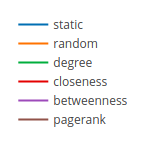
\includegraphics[scale=0.78]{pics/colormap.png}
\end{center}

	\begin{figure}
		\centering
		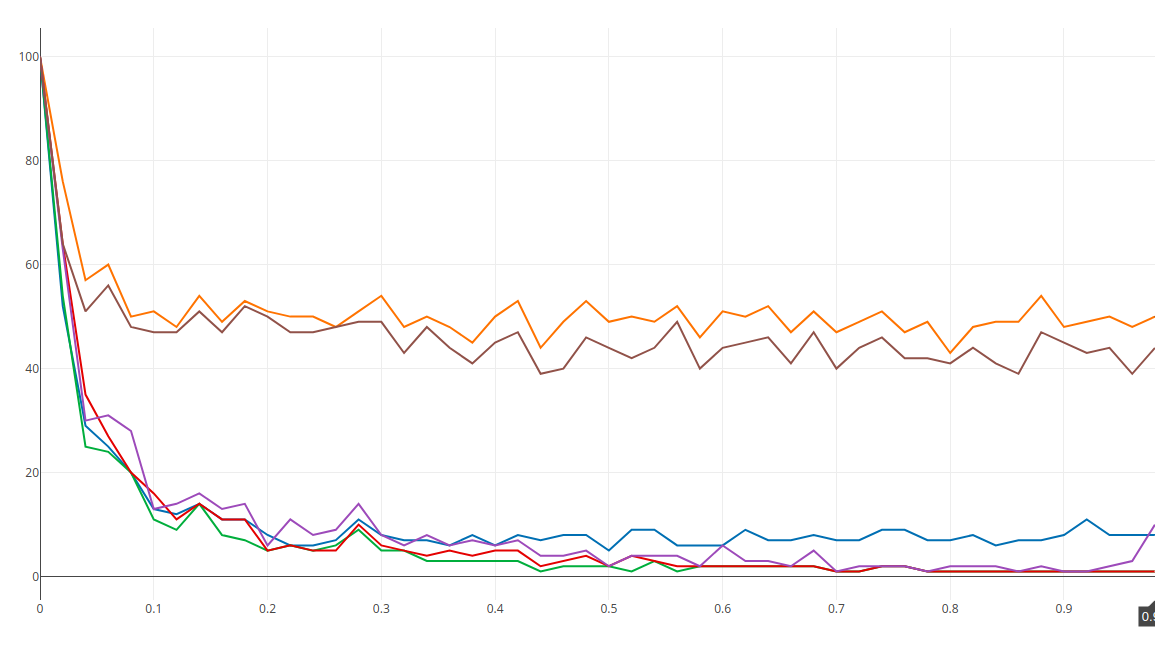
\includegraphics[width=\textwidth]{pics/random_count.png}
		\caption{Зависимость количества кластеров от вероятности в модели Эрдеша-Реньи при случайных весах ребер.}
		\label{fig:c_er_r}
	\end{figure}
	
	\begin{figure}
		\centering
		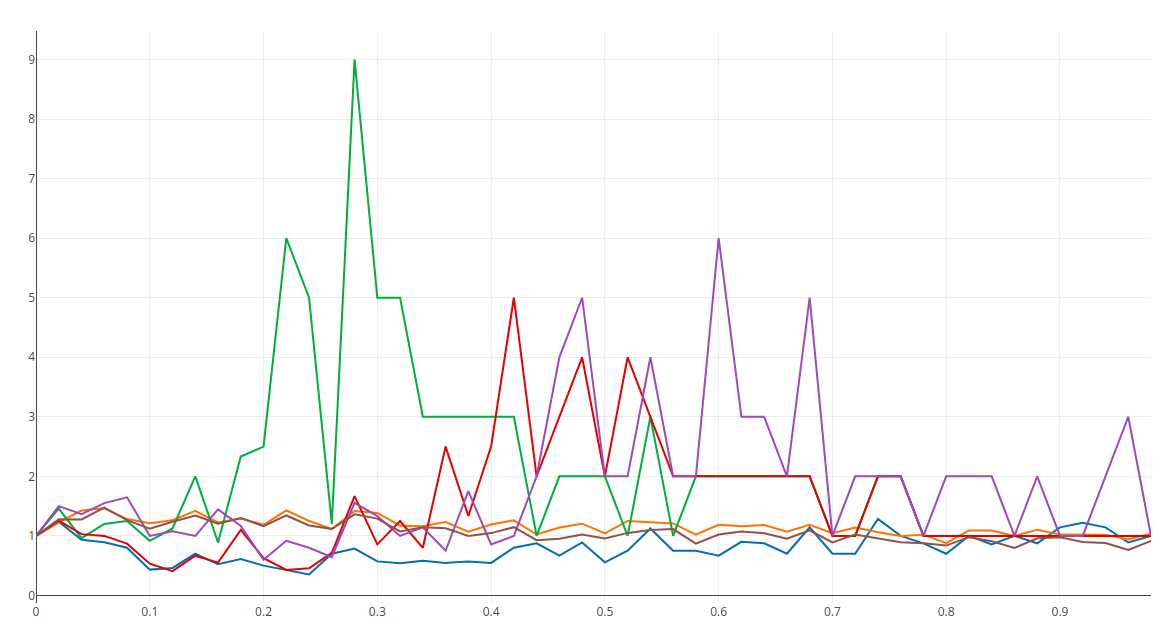
\includegraphics[width=\textwidth]{pics/random_d.png}
		\caption{Зависимость $c_{dir}/c_{undir}$ от вероятности в модели Эрдеша-Реньи при случайных весах ребер.}
		\label{fig:cc_er_r}
	\end{figure}
	
	\begin{figure}
		\centering
		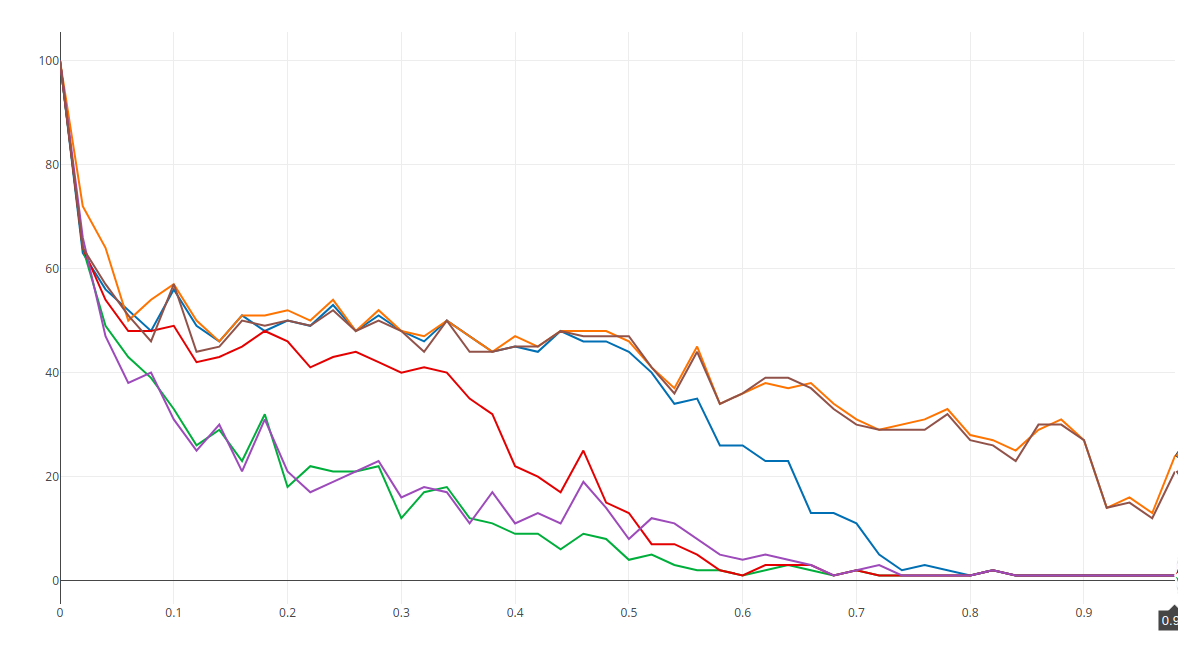
\includegraphics[width=\textwidth]{pics/jaccard_count.png}
		\caption{Зависимость числа сообществ от вероятности в модели Эрдеша-Реньи при весах ребер, равных индексу Жаккара.}
		\label{fig:c_er_j}
	\end{figure}

	\begin{figure}
		\centering
		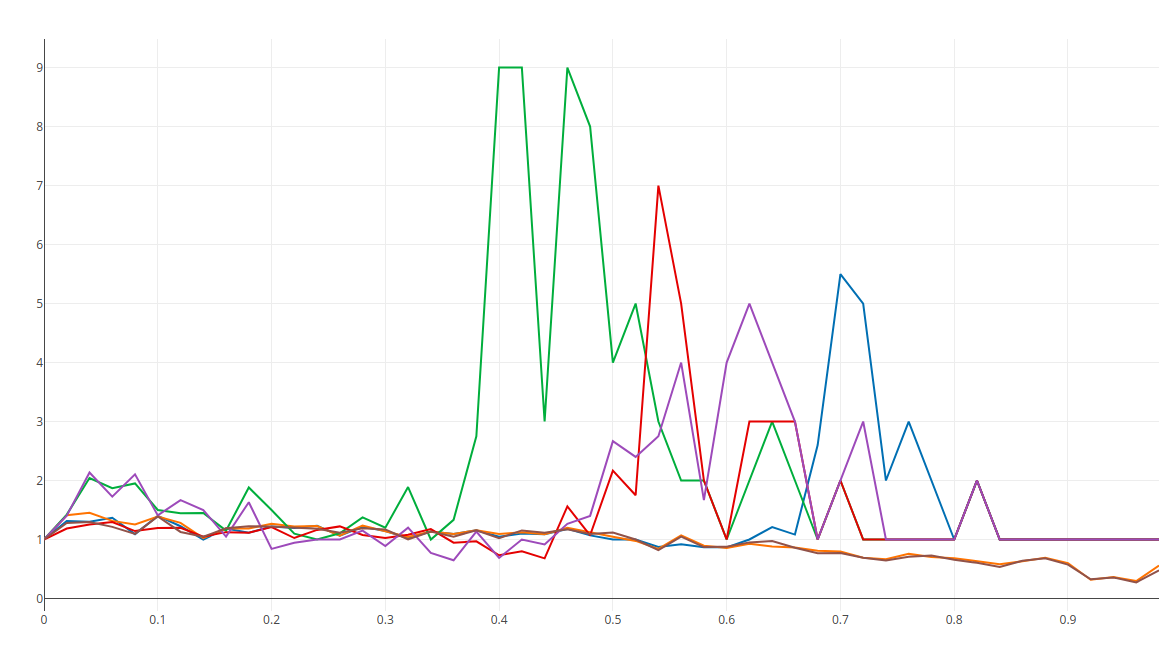
\includegraphics[width=\textwidth]{pics/jaccard_d.png}
		\caption{Зависимость $c_{dir}/c_{undir}$ от вероятности в модели Эрдеша-Реньи при весах ребер, равных индексу Жаккара.}
		\label{fig:cc_er_j}
	\end{figure}
	
Видно, что с увеличением вероятности количество кластеров для всех центральностей и весов ребер уменьшается. При отсутствии ребер вершины не объединяются, и число кластеров равно 100. Оно уменьшается до 1 (то есть, полный граф наш алгоритм объединяет в один кластер) при использовании центральностей static, degree, closeness, betweenness. Если использовать центральности random или pagerank, количество кластеров всегда остается сильно больше единицы.\\
	
По графикам зависимости $c_{dir}/c_{undir}$ можно заметить, что при некоторых промежуточных вероятностях число кластеров в ориентированном графе сильно выше, чем в неориентированном. При этом такой эффект начинается при вероятностях, больших критической $p_{c}=\frac{\ln 100}{100}\approx 0.05$ в 4-10 раз, то есть граф уже достаточно сильно связен. Это явление нужно исследовать более подробно, чему будет посвящен следующий раздел.\\

\subsection{Граф Барабаши-Альберт}

\begin{figure}[h!]
	\centering
	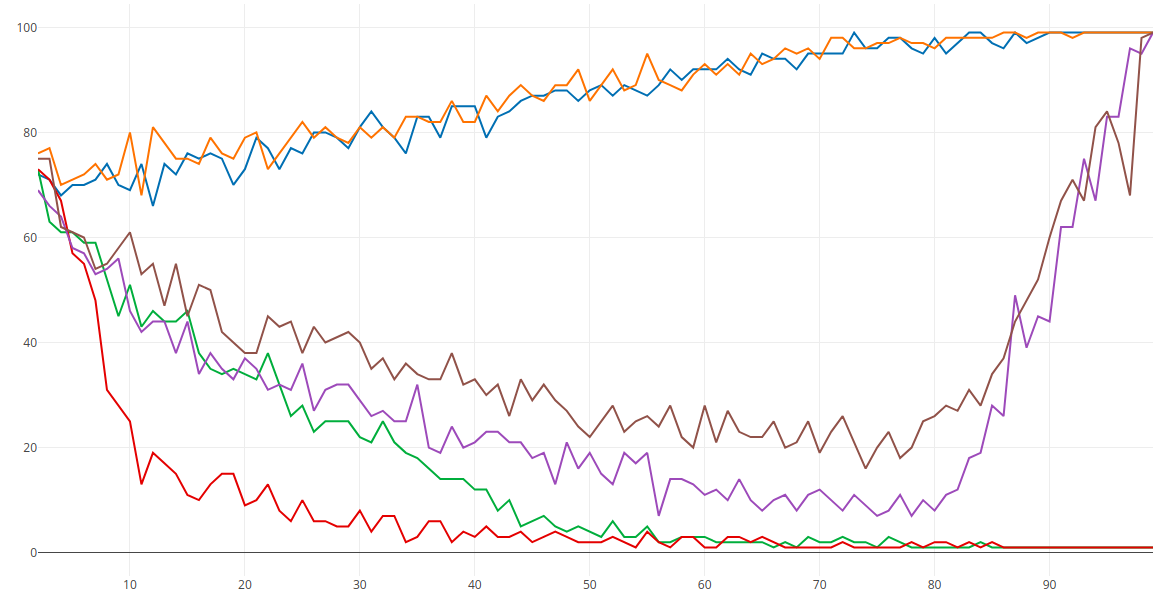
\includegraphics[width=\textwidth]{pics/ba_static.png}
	\caption{Зависимость количества кластеров от числа генерируемых ребер в модели Барабаши-Альберт при весах ребер, равных $1/2$.}
	\label{fig:c_ba_s}
\end{figure}

Здесь в экспериментах мы непосредственно увеличиваем число генерируемых ребер. Полученные графики \ref{fig:c_ba_s}, \ref{fig:cc_ba_s}, \ref{fig:c_ba_j}, \ref{fig:cc_ba_j} при некоторых параметрах показывают те же результаты для количества кластеров и отношения количеств кластеров в ориентированном и неориентированном графе, что и в модели Эрдеша-Реньи. Для некоторых параметров зависимости пока трудно понять. Например, при весах всех ребер и вершин, равных $1/2$, количество кластеров почти монотонно растет. Но для большинства параметров сохраняется упомянутый эффект, состоящий в том, что при некоторой промежуточной плотности ребер кластеризация ориентированных и неориентированных графов принципиально различается.

\begin{figure}[h!]
	\centering
	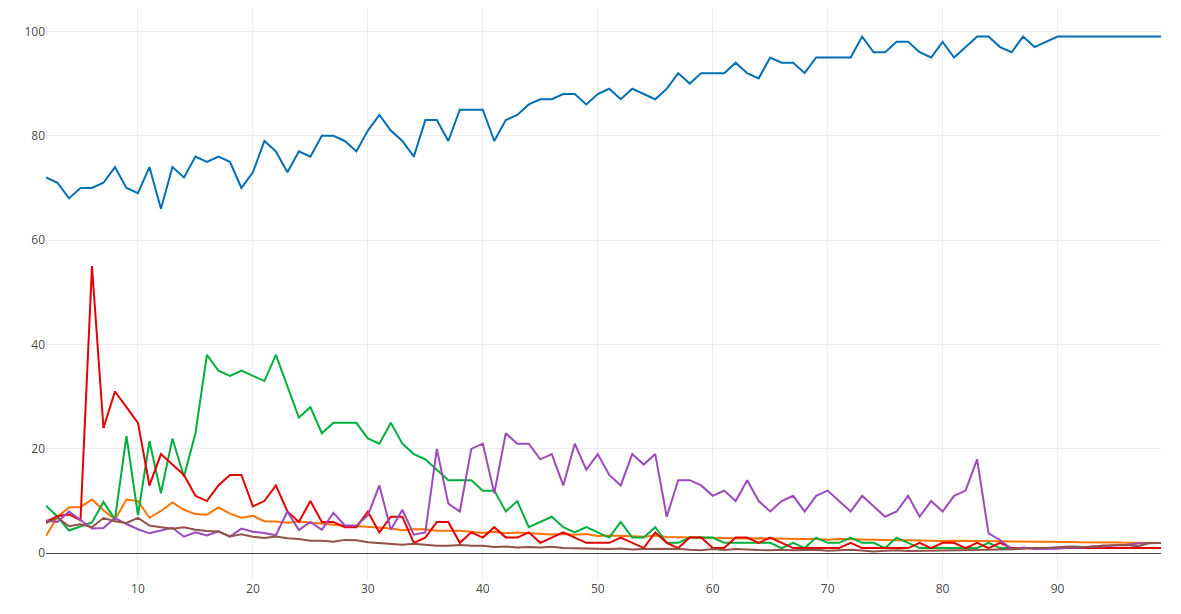
\includegraphics[width=\textwidth]{pics/ba_static_d.png}
	\caption{Зависимость $c_{dir}/c_{undir}$ от числа генерируемых ребер в модели Барабаши-Альберт при весах ребер, равных $1/2$.}
	\label{fig:cc_ba_s}
\end{figure}

\begin{figure}[h!]
	\centering
	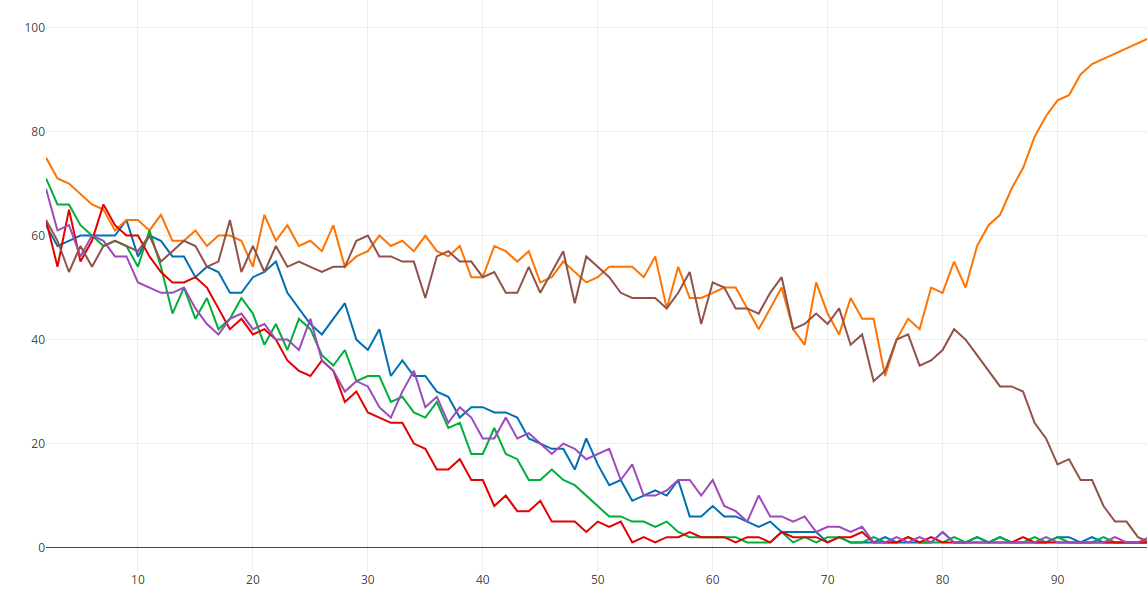
\includegraphics[width=\textwidth]{pics/ba_jaccard.png}
	\caption{Зависимость количества кластеров от числа генерируемых ребер в модели Барабаши-Альберт при весах ребер, равных индексу Жаккара.}
	\label{fig:c_ba_j}
\end{figure}

\begin{figure}[h!]
	\centering
	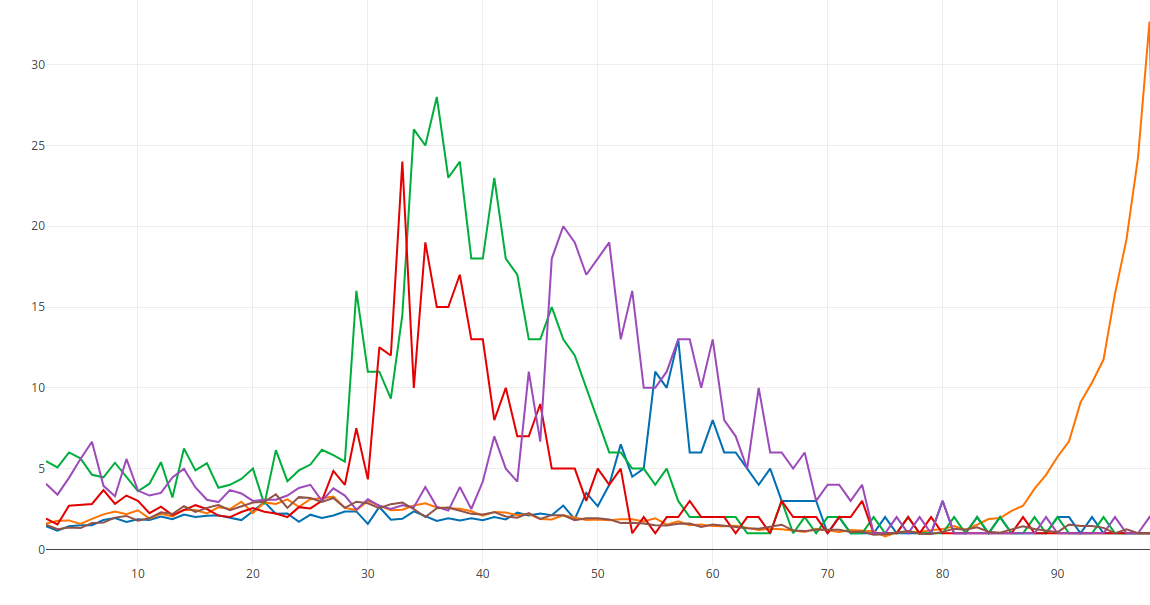
\includegraphics[width=\textwidth]{pics/ba_jaccard_d.png}
	\caption{Зависимость $c_{dir}/c_{undir}$ от числа генерируемых ребер в модели Барабаши-Альберт при весах ребер, равных индексу Жаккара.}
	\label{fig:cc_ba_j}
\end{figure}

\newpage
\section{Контролируемое изменение ориентации ребер}
Попытаемся изучить подробнее эффект, замеченный в предыдущем разделе (4.1.1).\\

В этом разделе будем исследовать граф Эрдеша-Реньи. Попробуем понять, почему, когда ребра становятся ориентированными, число кластеров заметно увеличивается. Проведем эксперимент к контролируемым изменением типа ребер. Построим эксперимент следующим образом:

\begin{enumerate}
	\item Зафиксируем некоторое промежуточное значение вероятности, при котором эффект увеличения числа кластеров будет наблюдаться. 
	
	\item Сгенерируем \textit{неориентированный невзвешенный} граф с помощью модели Эрдеша-Реньи. Представим граф симметричной матрицей смежности.
	
	\item Будем в случайном порядке "ориентировать"\ каждое ребро. А именно, запишем все пары вершин, между которыми есть неориентированное ребро, в список. Пока список не пуст, будем выбирать случайное ребро $(i, j)$ из списка, после чего удалять одну из единиц в позиции $(i,j)$ или $(j,i)$ из матрицы смежности. Позицию для удаления будем также выбирать случайно. После этого ребро из списка нужно удалить, чтобы ребро не исчезло из графа совсем, а только "ориентировалось".
	
	\item После каждой операции удаления единицы из матрицы смежности (или после нескольких таких операций, если граф большой) будем кластеризовать граф заново и смотреть, что меняется.
	
\end{enumerate}

\subsection{Увеличение количества кластеров}
На рисунке \ref{fig:interpolation} синим цветом изображена зависимость числа кластеров при фиксированных весах ребер и вершин, равных $1/2$. Каждая точка получена усреднением по 100 случайным графам Эрдеша-Реньи.\\

На самом деле, возрастание числа кластеров нетрудно объяснить. Чтобы образовался кластер $C_1$ размера $|C_1|=F+1$, необходимо, чтобы уже существовал кластер $C$ размера $|C|=F$, и, вместе с тем, существовала вершина $v$, желающая присоединиться к нему. Кроме того, кластеру должно быть выгодно принять эту вершину, следовательно, должно быть ребро из некоторой вершины кластера в данную вершину $v$. Рассмотрим, как меняется эта ситуация при "ориентации"\ ребер. \\

Пусть $|V|=N$, $|E|=m_0$. Пусть есть кластер $C$ размера $F$. Для начала оценим, сколько вообще ребер находится в "разрезе"\ между этим кластером и оставшимися вершинами, то есть, сколько ребер соединяет множества $C$ и $V/C$. В модели Эрдеша-Реньи среднее число таких ребер есть $F(N-F)p$. Будем называть это число \textit{степенью} всего множества $C$. Будем различать in- и out-степень (число ребер, исходящих из $C$ и входящих в $C$ соответственно), обозначим их $d_0^{in}$, $d_0^{out}$. Изначально все ребра неориентированные, поэтому $d_0^{in}= d_0^{out}=F(N-F)p$. Вычислим $d_i^{in}$ и $d_i^{out}$ - соответствующие степени после ориентиции $i$ ребер.\\

Рассмотрим первый шаг алгоритма. Так как изменяемое ребро выбирается случайно, вероятность выбрать ребро из "разреза"\ есть $\frac{d^{in}_0}{m_0}$. Вероятность выбора определенного направления равна $\frac{1}{2}$. То есть, количество in-ребер множества $C$ с вероятностью $\frac{d_0^{in}}{2m_0}$ уменьшается на 1, а с вероятностью $1-\frac{d_0^{in}}{2m_0}$ остается тем же. То же происходит с количеством out-ребер $d_0^{out}$:

\begin{equation}
	d_1^{in}=\frac{d_0^{in}}{2m_0}\cdot (d_0^{in}-1)+(1-\frac{d_0^{in}}{2m_0})\cdot d_0^{in} = d_0^{in}\cdot (1-\frac{1}{2m_0}).
\end{equation}

Тогда на $i$-м шаге:

\begin{equation*}
	d_i^{in}=d_0^{in}\cdot (1-\frac{1}{2m_0})\cdot(1-\frac{1}{2(m_0-1)})\cdot...\cdot (1-\frac{1}{2(m_0-i+1)}) =
\end{equation*}
\begin{equation}
	 =d_0^{in}\cdot\prod_{j=0}^{i-1}(1-\frac{1}{2(m_0-j)})\leq F(N-F)p\cdot(1-\frac{1}{pN(N-1)})^i,
\end{equation}

где $m_0=\frac{pN(N-1)}{2}$ - среднее число неориентированных ребер в начале алгоритма. На каждом шаге средние in- и out-степени умножаются на число, меньшее единицы.\\

Рассмотрим множество концов рассматриваемых in-ребер ($A_i^{in}$) и out-ребер ($A_i^{out}$) из "разреза"\, лежащих в $V/C$, на $i$-м шаге алгоритма. Заметим, что это мультимножества, причем $|A_i^{in}|=d_i^{in}$, $|A_i^{out}|=d_i^{out}$. Изначально $A_0^{in}=A_0^{out}$. На каждом шаге из этих множеств с некоторой вероятностью может удалиться один элемент, и уменьшение их мощности в среднем описывается формулой (21). Вершины, которые могут присоединиться к кластеру $C$ на $i$-м шаге алгоритма, должны лежать в $A_i^{in}\cap A_i^{out}$, которое, если одинаковых элементов в мультимножествах не слишком много (то есть, вероятность $p$ не слишком большая, а значит, и степени вершин тоже), с увеличением $i$ постепенно уменьшается. Это означает, что с каждым шагом алгоритма все меньше вершин смогут присоединиться к кластеру $C$, что будет уменьшать его мощность.\\

Если один из экземпляров вершины был удален из одного множества, то из второго он уже не будет удаляться (так поставлен эксперимент, нет смысла полностью удалять ребра из графа). Если в графе много ребер, то увеличиваются и степени вершин, а значит, мощность пересечения $A_i^{in}\cap A_i^{out}$ не уменьшается так сильно: чем больше изначально соседей у вершины $v$, тем больше вероятность, что после $i$ шагов алгоритма найдется пара ребер, смежных с $v$, ориентированных в разные стороны. Эти рассуждения объясняют возрастание числа кластеров при ориентации ребер при некоторых промежуточных вероятностях $p$ и прекращение этого явления при больших вероятностях, что мы и наблюдали в предыдущем разделе.\\

Порядок роста числа кластеров удалось оценить только численно. Интерполяция для случая $p=1/2$ показана на рисунке \ref{fig:interpolation}. Для подбора коэффициентов использовался метод наименьших квадратов. Использовался полином $\alpha x^{\beta}+\gamma$ (показан зеленым цветом). Результаты: $\alpha \approx 6\cdot 10^{-15}$, $\beta \approx 4.5$, $\gamma \approx 12$. 

\begin{figure}[h!]
	\centering
	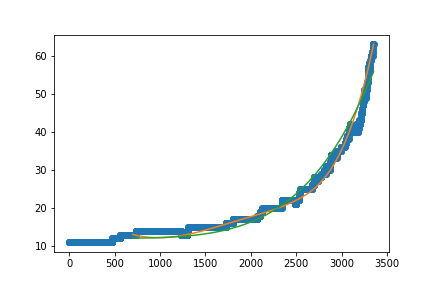
\includegraphics[width=\textwidth]{pics/interpolation.png}
	\caption{Интерполяция зависимости количества кластеров от номера итерации алгоритма. Граф строился на 270 вершинах. На итерации $i$ "ориентировано"\ $5\cdot i$ ребер. Вероятность проведения ребра равна $1/2$.}
	\label{fig:interpolation}
\end{figure}

\subsection{Распределение по количеству кластеров}
Рисунок \ref{fig:interpolation} отражает изменение среднего по ансамблю значения числа кластеров. Но также эта величина должна иметь дисперсию, так как дисперсию имеет число ребер графа, а число кластеров, как мы уже выяснили, зависит от числа ребер. Можно посмотреть на распределение по количеству кластеров в ансамбле в целом (рисунок \ref{fig:distribution}).

\begin{figure}[h!]
	\centering
	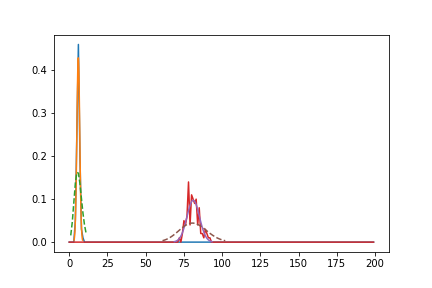
\includegraphics[width=\textwidth]{pics/distribution.png}
	\caption{Оценка распределений по числу кластеров для неориентированного (показан слева, синим цветом) и ориентированного (показан справа, красным цветом) графа, полученного в конце алгоритма. Граф строился на 250 вершинах. Вероятность проведения ребра равна $1/2$. Желтым и фиолетовым цветом показаны нормальные распределения, параметры которых оценены методом максимального правдоподобия ($\mu_{undir}=5.94$, $\sigma^2_{undir}=0.93$, $\mu_{dir}=81.07$, $\sigma^2_{undir}=4.10$). Пунктиром показаны распределения Пуассона.} 
	\label{fig:distribution}
\end{figure}

С помощью тестов Шапиро и Харке-Бера проверена нормальность данных. Полученные с помощью теста Шапиро p-value составили примерно $0.09$ для неориентированного графа и $0.08$ для ориентированного (использовался ансамбль из 30 графов, чтобы критерий был применим). Критерий Харке-Бера для выборки из 100 элементов дал результат $0.3$ для неориентированного и $0.2$ для ориентированного графа. Гипотезу нормальности во всех случаях можно принять.\\

Также на рисунке \ref{fig:distribution} видно увеличение дисперсии количества кластеров для ориентированного графа. Это можно объяснить тем, что в ориентированном графе при фиксированном количестве ребер может появиться гораздо больше различных вариантов топологий, чем в неориентированном.\\

\subsection{Распределение по размерам кластеров}
Посмотрим, как меняется распределение по размерам кластеров при добавлении ориентации ребрам (рисунок \ref{fig:d1234}). 

\begin{figure}[h!]
	\centering
	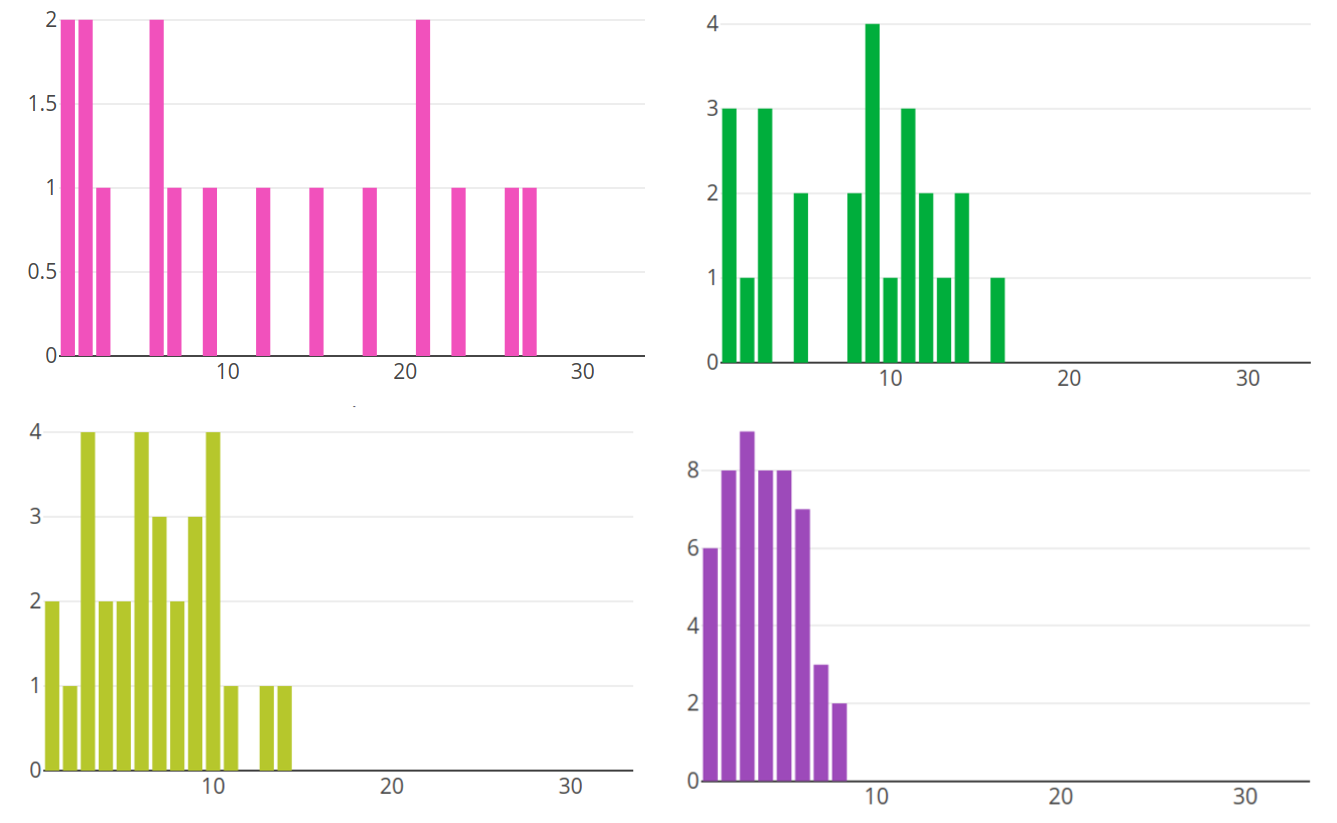
\includegraphics[width=\textwidth]{pics/d1234.png}
	\caption{Изменение распределений по размерам кластеров с увеличением количества ориентированных ребер. Вероятность проведения ребра равна $1/2$. Используется мера центральности Degree. Граф построен на 200 вершинах. Число ориентированных ребер увеличивается слева направо и сверху вниз и равно соответственно 700 (слева вверху), 4900 (справа вверху), 6100 (слева внизу), 8300 (справа внизу). Средний размер кластера равен соответственно 11.8, 8, 7, 4.} 
	\label{fig:d1234}
\end{figure}

Средний размер кластера уменьшается, что согласуется с результатом о том, что число кластеров увеличивается. Попробуем оценить полученное распределение.  Попробуем взять не слишком большую вероятность (здесь критическая вероятность 0.015) и достаточно большой граф (рисунок \ref{fig:d12}).

\begin{figure}[h!]
	\centering
	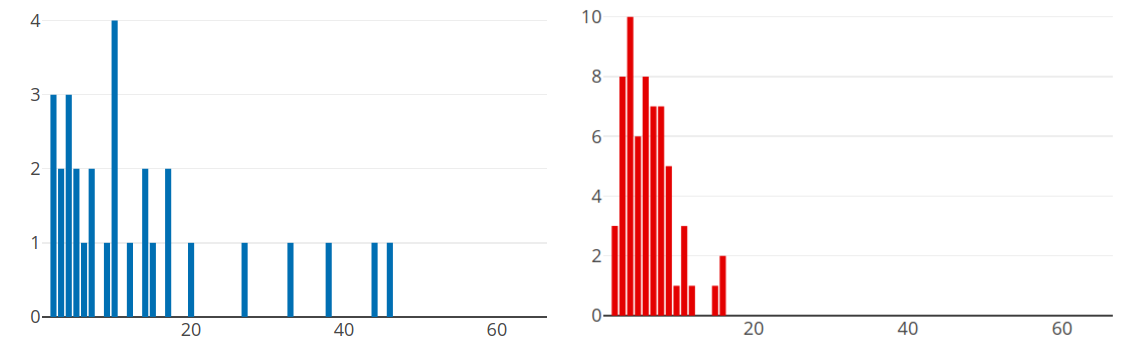
\includegraphics[width=\textwidth]{pics/d12.png}
	\caption{Распределение по размерам кластеров для неориентированного (слева) и ориентированного (справа) графа. Вероятность проведения ребра равна $1/40=0.025$. Используется мера центральности Degree. Граф построен на 400 вершинах.} 
	\label{fig:d12}
\end{figure}

Попробуем приблизить полученные распределения распределениями Пуассона, посчитав параметры $\lambda$ с помощью оценки максимального правдоподобия. Будем использовать QQ-графики (рисунок \ref{fig:qqs}). Как видно уже из гистограмм, распределения смещены от теоретических влево, причем для неориентированного графа достаточно сильно. Это явление мы и наблюдаем на QQ-графиках.

\begin{figure}[h!]
	\centering
	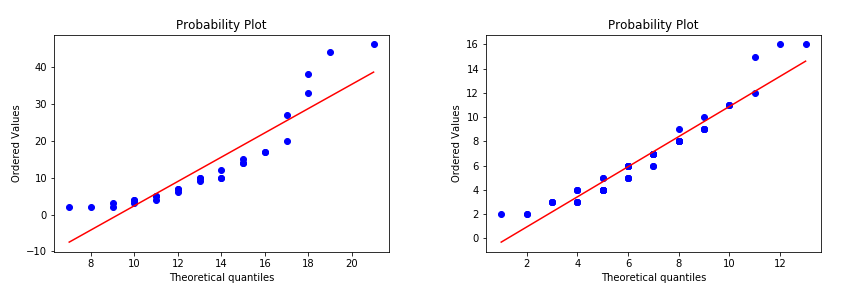
\includegraphics[width=\textwidth]{pics/qqs.png}
	\caption{Приближение распределений по размерам кластеров для неориентированного (слева) и ориентированного (справа) графа с помощью распределений Пуассона. Вероятность проведения ребра равна $1/40$. Используется мера центральности Degree. Граф построен на 400 вершинах. Средние равны соответственно 13.3 и 6.5.} 
	\label{fig:qqs}
\end{figure}

\section{Исследование модулярности}
В теоретическом введении была введена модулярность для ориентированного графа и объяснено ее значение. Проверим, что будет происходить с модулярностью в нашем случае. Будем максимизировать модулярность жадным образом. Графы будем генерировать с помощью модели Эрдеша-Реньи. Для получения большого количества графов будем варьировать вероятность. Рассмотрим две центральности: betweenness и PageRank. Полученные зависимости изображены на рисунке \ref{fig:greedy_mod}. \\

\begin{figure}[h!]
	\centering
	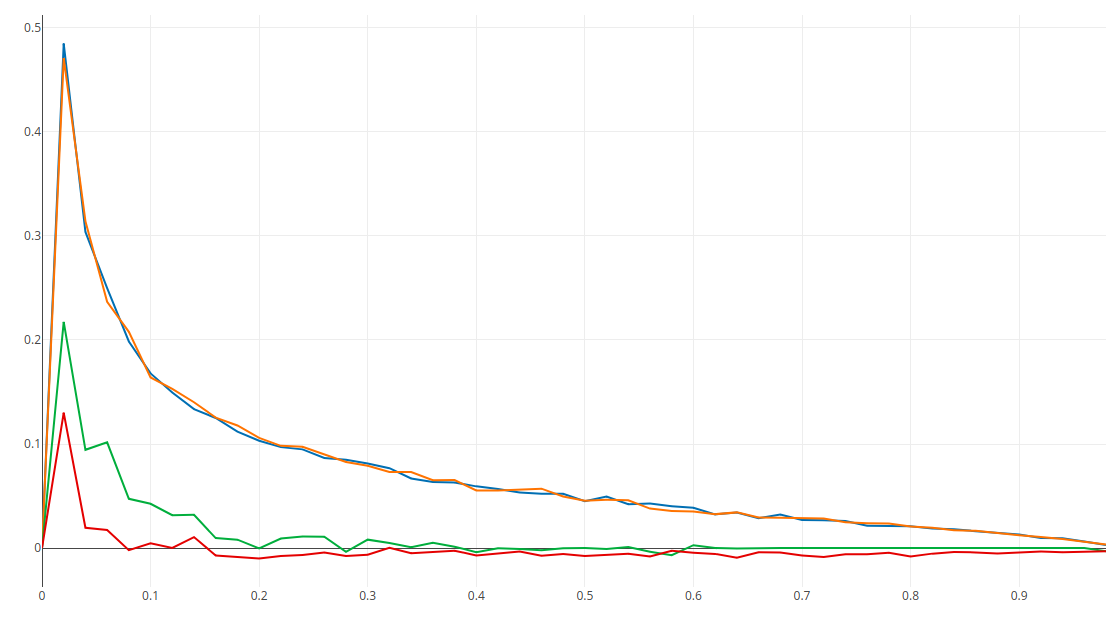
\includegraphics[width=\textwidth]{pics/greedy_mod.png}
	\caption{Зависимость модулярности разбиения ориентированного и максимальной модулярности от вероятности в модели Эрдеша-Реньи. Красным и зеленым обозначена модулярность разбиения, получаемого с помощью изучаемого алгоритма, с использованием центральностей PageRank и betweenness соответственно. Желтым и синим показана максимальная модулярность (она, вообще говоря, от центральностей не зависит).} 
	\label{fig:greedy_mod}
\end{figure}

Модулярность разбиения, получаемого с помощью нашего алгоритма, ниже максимальной, но ее зависимость от вероятности ведет себя похожим образом. Возможно, различие можно объяснить тем, что в нашем алгоритме агенты принимают решение, основываясь не только на плотности связей и весе ребер, но и на том, какой вес имеет рассматриваемая вершина. При использовании центральности betweenness большой вес дается вершинам, лежащим на большом количестве кратчайших путей между другими вершинами. Такие вершины имеют много in- и out-соседей, и любые ребра, смежные с ними, не вносят большого вклада в модулярность. При этом из-за большого веса этих вершин их in-соседи будут стремиться оказаться с ними в одном кластере, и это будет (отчасти) кластеризация по плотности связей. При использовании центральности PageRank большой вес имеют вершины с большим количеством in-соседей, а out-соседей у них может быть мало. Так, ребро, исходящее из этой вершины, может вносить большой вклад в модулярность, но при этом вершина, на которую "ссылается"\ вершина с большим весом, будет также иметь большой вес, а значит, скорее всего, рассматриваемое out-ребро окажется внутри кластера. Таким образом, модулярность при использовании PageRank действительно окажется меньше модулярности, полученной при использовании betweenness, и обе они окажутся меньше максимальной.